% !TeX spellcheck = en_US
\documentclass[12pt,fleqn]{article}


\usepackage[english]{babel}

\usepackage{texfiles/SpeedyGonzales}
\usepackage{texfiles/MediocreMike}
\usepackage{multicol}



\title{\vspace*{-3.5cm}Bayesian Optimization for Hyperparameter Tuning in The Fully Connected Layers of VGG16}
\author{Søren Winkel Holm\and Oskar Wiese\and Anders Henriksen\and Anne Agathe Pedersen}
\date{\today}

\fancypagestyle{plain}
{
	\fancyhf{}
	\rfoot{Page \thepage{} of  \pageref{LastPage}}
	\renewcommand{\headrulewidth}{0pt}
}
%\pagestyle{fancy}
%\fancyhf{}
%\lhead{Lala}
%\chead{}
%\rhead{}
%\rfoot{Page \thepage{} of \pageref{LastPage}}

\graphicspath{{imgs/}}
\usepackage{float}
\usepackage[caption = false]{subfig}
%\linespread{1.15}

%TODO: \numberwithin{equation}{section}
%TODO: \numberwithin{footnote}{section}
%TODO: \numberwithin{figure}{section}
%TODO: \numberwithin{table}{section}

\begin{document}

\maketitle

%\tableofcontents
%\thispagestyle{fancy}
%\tableofcontents

\begin{abstract}
\noindent Optimization of neural network hyper parameters is a costly process of uncertainty balancing exploration of parameters and exploitation of known results. This experiment compares Bayesian Optimization using Gaussian Processes to  simple grid search for finding the optimal hyperparameters for the fully-connected layers of the VGG16 image classification deep convolutional network. The success of the training is compared for three different acquisitions functions. Little difference is found which could be a result of the limited scope of the network training but the Bayesian Optimization method allows for a visualization of the estimated model accuracy on the hyper parameter space.

\end{abstract}

\begin{multicols}{2}


\section{Introduction} 
Development of effective machine learning models has spawned a vision of generalizable machine intelligence, which can replace slower and more erroneous human work in many fields. While this generalizability is often true, the popular deep models have at least one obvious issue that requires domain knowledge, skill and large amounts of computing power to overcome; hyperparameter optimization. Optimizing the hyperparameters can usually devolve into random guessing or extensive sampling from a large parameter space. Bayesian Optimization guides this by modeling the parameter space, explicitly reducing the guessing and limiting the size of the search involved in finding the parameters with use of an acquisition function and probabilistic model.

In this project, Baysian optimization with Gaussian processes as probabilistic model will be used to optimize the hyperparameters for training the VGG16 network on the CIFAR10 image classification data set thus gaining experience with the method and comparing it to simple grid search.
\vspace*{-0.3cm}
\section{Methods}
\vspace*{-0.2cm}
\texttt{All code available at \url{github.com/sorenmulli/active_learning_cases}}

The objective function that is to be optimized consists of using the \texttt{pytorch} pretrained VGG16 network \cite{vgg} and training its three fully-connected layers on 8000 images from the CIFAR10 10-class dataset \cite{cifar10} for 10 epochs and returning the accuracy on the 2000 validation images. 
This accuracy is then modeled by the non-parametric Gaussian processes (GP) as a function of three following hyperparameters in the given ranges:
\vspace*{-0.05cm}
\begin{itemize}
	\item Number of units in the hidden layer \(\in [1, 5000]\) 
	\item Dropout probability before each layer \(\in [0,1]\)
	\item Activation function after each layer (\textit{tanh}, ReLU, ReLU6, Sigmoid)
\end{itemize}
The GP operates using the smoothness assumption on the network outputs, and its lengthscale and variance parameters are optimized using log-likelihood. The number of units are scaled down to \([0,1]\) for lengthscale convergence, and the categorical variable is one-out-of-4 encoded. 

From this probabilistic model, three different acquisition functions, that chooses parameters for next training and balances exploration and exploitation, are compared:

\begin{itemize}
	\item \textbf{Expected Improvement (EI)} maximizing the accuracy improvement for each possible hyper parameter
	\item \textbf{Maximum Probability of Improvement (MPI)} training the network with the parameters most likely to obtain a higher accuracy
	\item \textbf{Upper Confidence Bound(UCB)} Using the mean and standard deviation from the GP directly to guide the exploration
\end{itemize}
The Bayesian optimization is started by sampling five random points from the objective function, fitting the GP to these and iteratively surveying the next 7 points in the hyperparameter space using the GP and the acqusistion function. This is done for each acqusition function together with a grid search of equally spaced point in the chosen hyper parameter domain, resulting in \(4\times12\) iterations over the network. The optimization is performed by the GPyOpt library \cite{gpyopt} with the  explore/exploit trade-off variable set to 0.01.

For each method, the optimal parameters are stored and a network is trained and evaluated on the test set of 10000 images.

\end{multicols}
\vspace*{-0.3cm}
\section{Results}
\vspace*{-0.2cm}
\begin{table}[H]\label{resultater}
	\begin{tabular}{l|lllll}
		  & Hidden units & Dropout \textit{p} & Activation & Val. accuracy &Test accuracy \\ \hline
		BO: EI  & 2540      & 16\pro              & \textit{tanh}             &    62.8\pro & 61.7\pro   \\ 
		BO: MPI & 2403         & 61\pro             & Sigmoid             & 64.7\pro  & 63.1\pro     \\ 
		BO: UCB & 1150         & 53\pro              & Sigmoid             & 64.6\pro  & 64.4\pro     \\ 
		Grid search & 2000         & 66\pro              & Sigmoid             & 64.9\pro & 63.1\pro          \\
	\end{tabular}
	\caption{The optimal hyperparameters from running Bayesian optimization (BO) with all three acquisition functions as well as grid search. All iterations can be seen in the appendix.}
\end{table}
\begin{figure}
	\centering
	
	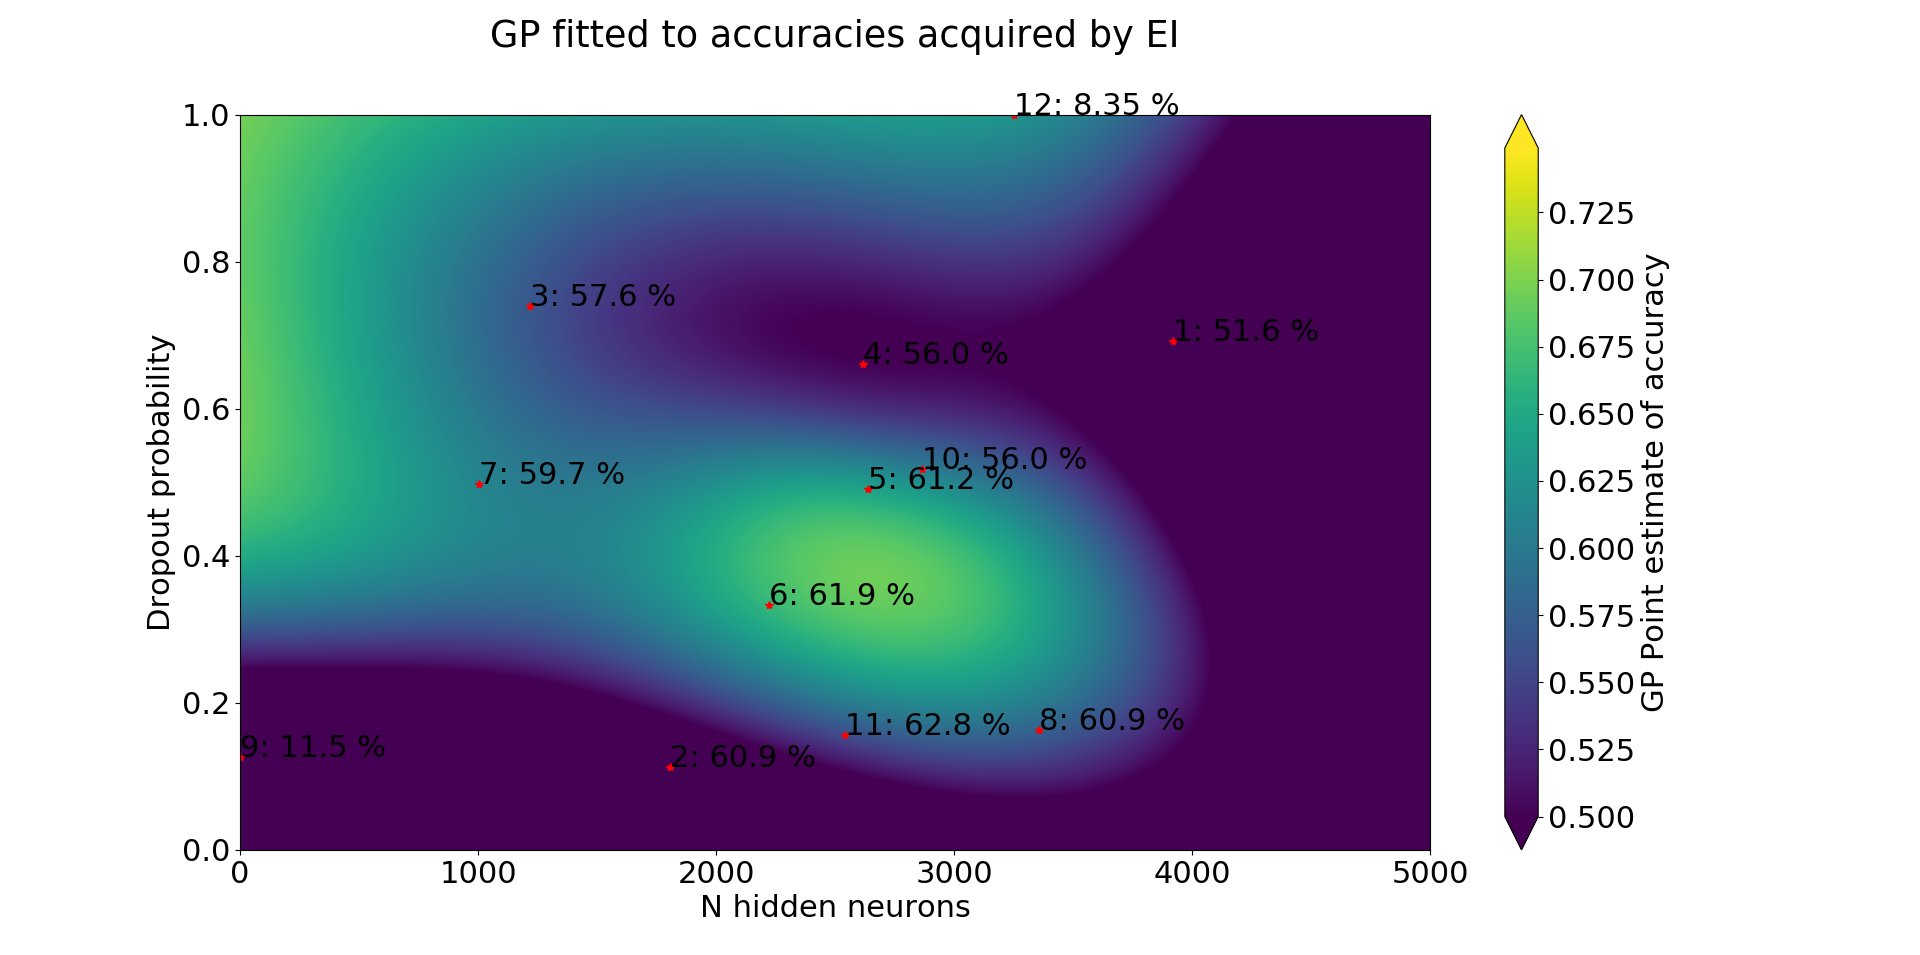
\includegraphics[width=\textwidth]{EIGP}	
	
	\caption{The Gaussian process fitted to the twelve accuracy points acquired by the expected improvement function. The other GP visualizations can be seen in the appendix.}
	\label{fig:gp}
	%It is clear that especially the sixth iteration of the grid search happens to hit points where the GP finds accuracy peaks. 
\end{figure}

\begin{multicols}{2}
\vspace*{-1.6cm}
\section{Discussion}
%In this section you interpret your findings and describe why they are important and how they fit in with
%other research. You can also mention ways your study could have been improved and future areas of
%research.
% What might the answer imply, and what does it matter?
% How does it fit in with what other researchers have found?
% What are the perspectives for future research? 
\vspace*{-0.2cm}
The differences in accuracies between the model proposed by the Bayesian optimization models and grid search are very small \(\delta \sim 1\pro \) and convincing statistical significance is not expected. In this case, the grid search results are as good as the Bayesian optimization scheme. This GP, however, allows for visualization of the shape of the objective function such as fig \ref{fig:gp} and in the appendix, where common sense choices such as \(p\sim 40\pro \) and a fairly high amount of hidden neurons are suggested as a maximum. From the other appendix visualizations, the other acqusition functions show a more exploitative approach than the expected improvement.

Each training only consisting of ten epochs, so the effect of the hyperparameters might not have enough time to influence the accuracy. This could result in a weak smoothness assumption and therefore a GP that might not be accurate enough after twelve data points. This short amount of training time also results in the optimization having to find parameters that make VGG16 converge fast, which might not generally be an optimal way of finding the best parameters for a larger training session. It is thus an interesting task to scale this experiment to a large training session or implementing the number of epochs as a tunable hyper-parameter.  

The results found in this study does not fit in with what other researches have found. Other studies have found that BO find state of the art hyperparameters for several different Machine Learning algorithms. \cite{baylearn, baylearn2} 

%As each training only consisting of ten epochs, the effect of the hyperparameters might not have enough time to influence the accuracy for the smoothness assumption to be strong enough for the GP to be accurate after twelve data points.
\vspace*{-0.3cm}
\section{Learning outcome}

Though better performance of Bayesian optimization could not be shown, the project yielded experience in using a well-defined hyperparameter searching scheme. It has become obvious that for setting up such a scheme, the convergence of the GP is key, as factors such as lengthscale normalization were important for getting sensible results. From the visualizations, it was learned that consideration of the explotation/exploration trade-off must be factored into the choice of acqusition method.

The promising method of exploring parts of a complex parameter space instead of an exhaustive search makes Bayesian optimization an important part of the model fitting toolbox.


\end{multicols}

\begin{thebibliography}{9}
	\bibitem{vgg} Simonya, K, Zisserman, A.: " Very Deep Convolutional Networks for Large-Scale Image Recognition.", ICLR: 2015, at: \url{https://arxiv.org/pdf/1409.1556.pdf}
	\bibitem{cifar10} Krizhevsky, A.: "The CIFAR-10 dataset", at \url{https://www.cs.toronto.edu/~kriz/cifar.html}
	\bibitem{gpyopt} Machine Learning Group, University of Sheffield: "GPyOpt’s documentation", at \url{https://gpyopt.readthedocs.io}
	\bibitem{baylearn} Adams, Ryan P. et al: " Practical Bayesian Optimization of Machine Learning Algorithms ", 2012
	\bibitem{baylearn2} Swersky, Kevin and Snoek, Jasper and Adams, Ryan P. : " Multi-Task Bayesian Optimization ", 2013
\end{thebibliography}

\section{Appendix}
\begin{figure}[H]

		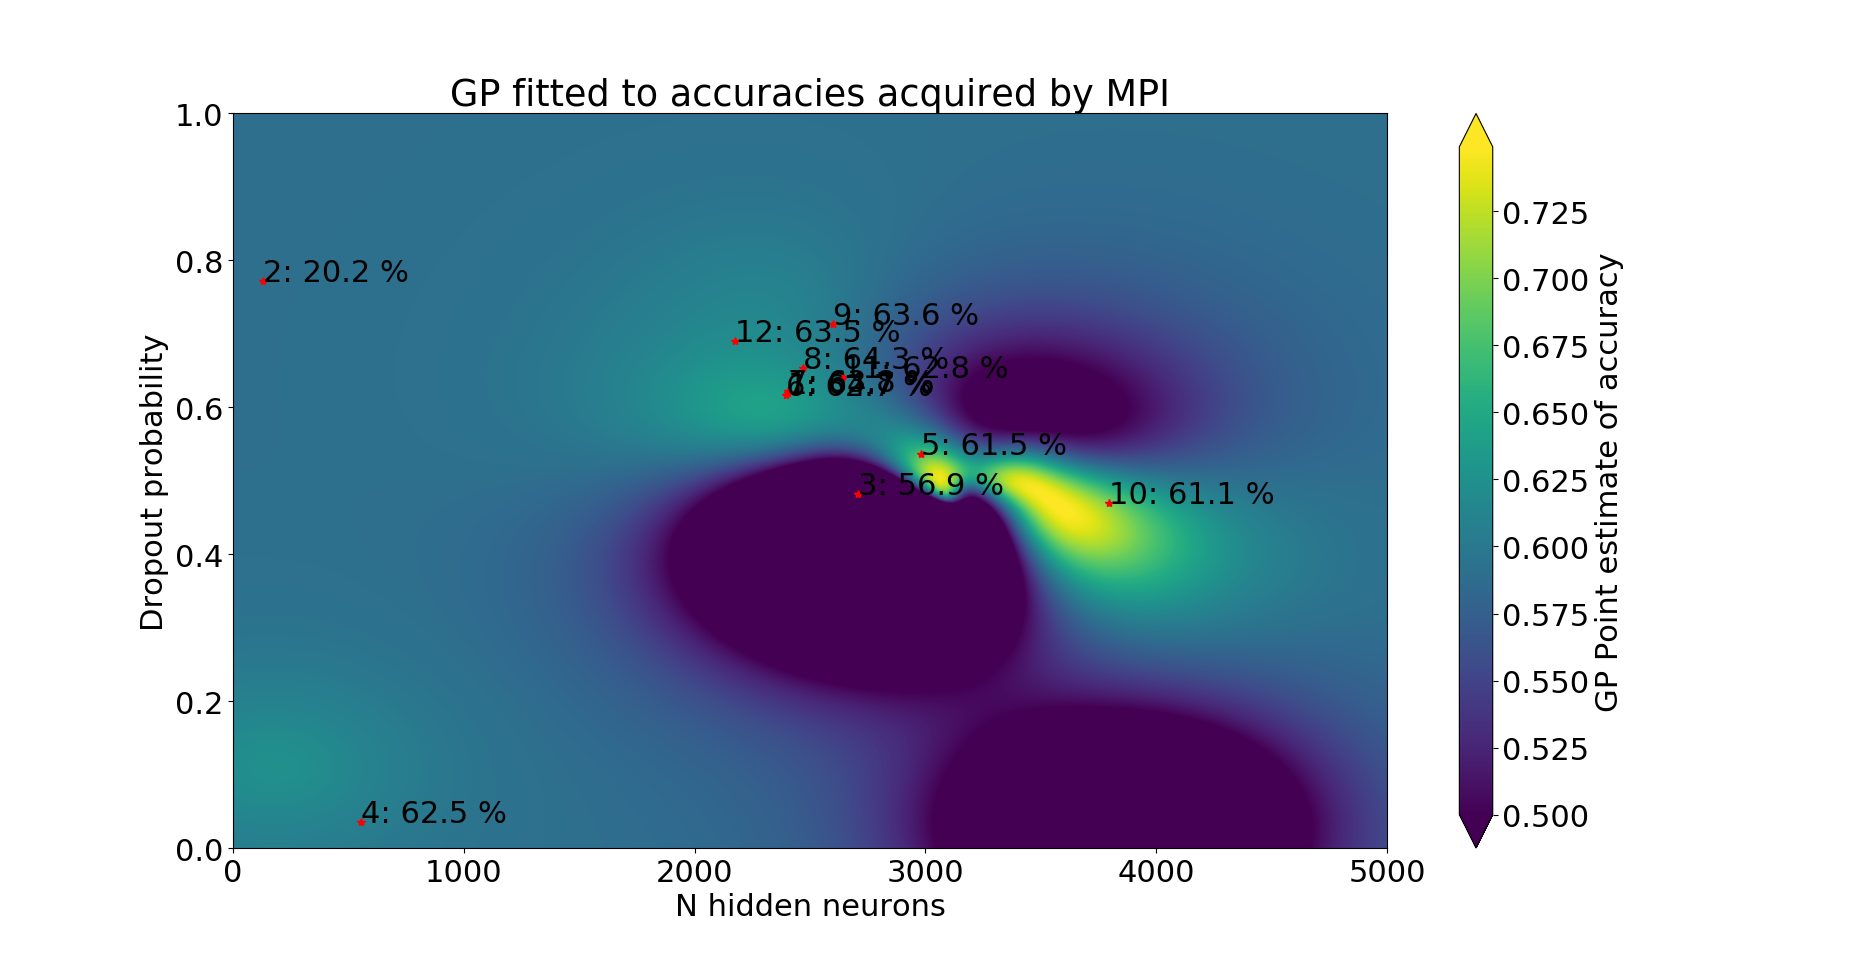
\includegraphics[width=\textwidth]{MPIGP}	
\end{figure}
\begin{figure}[H]
		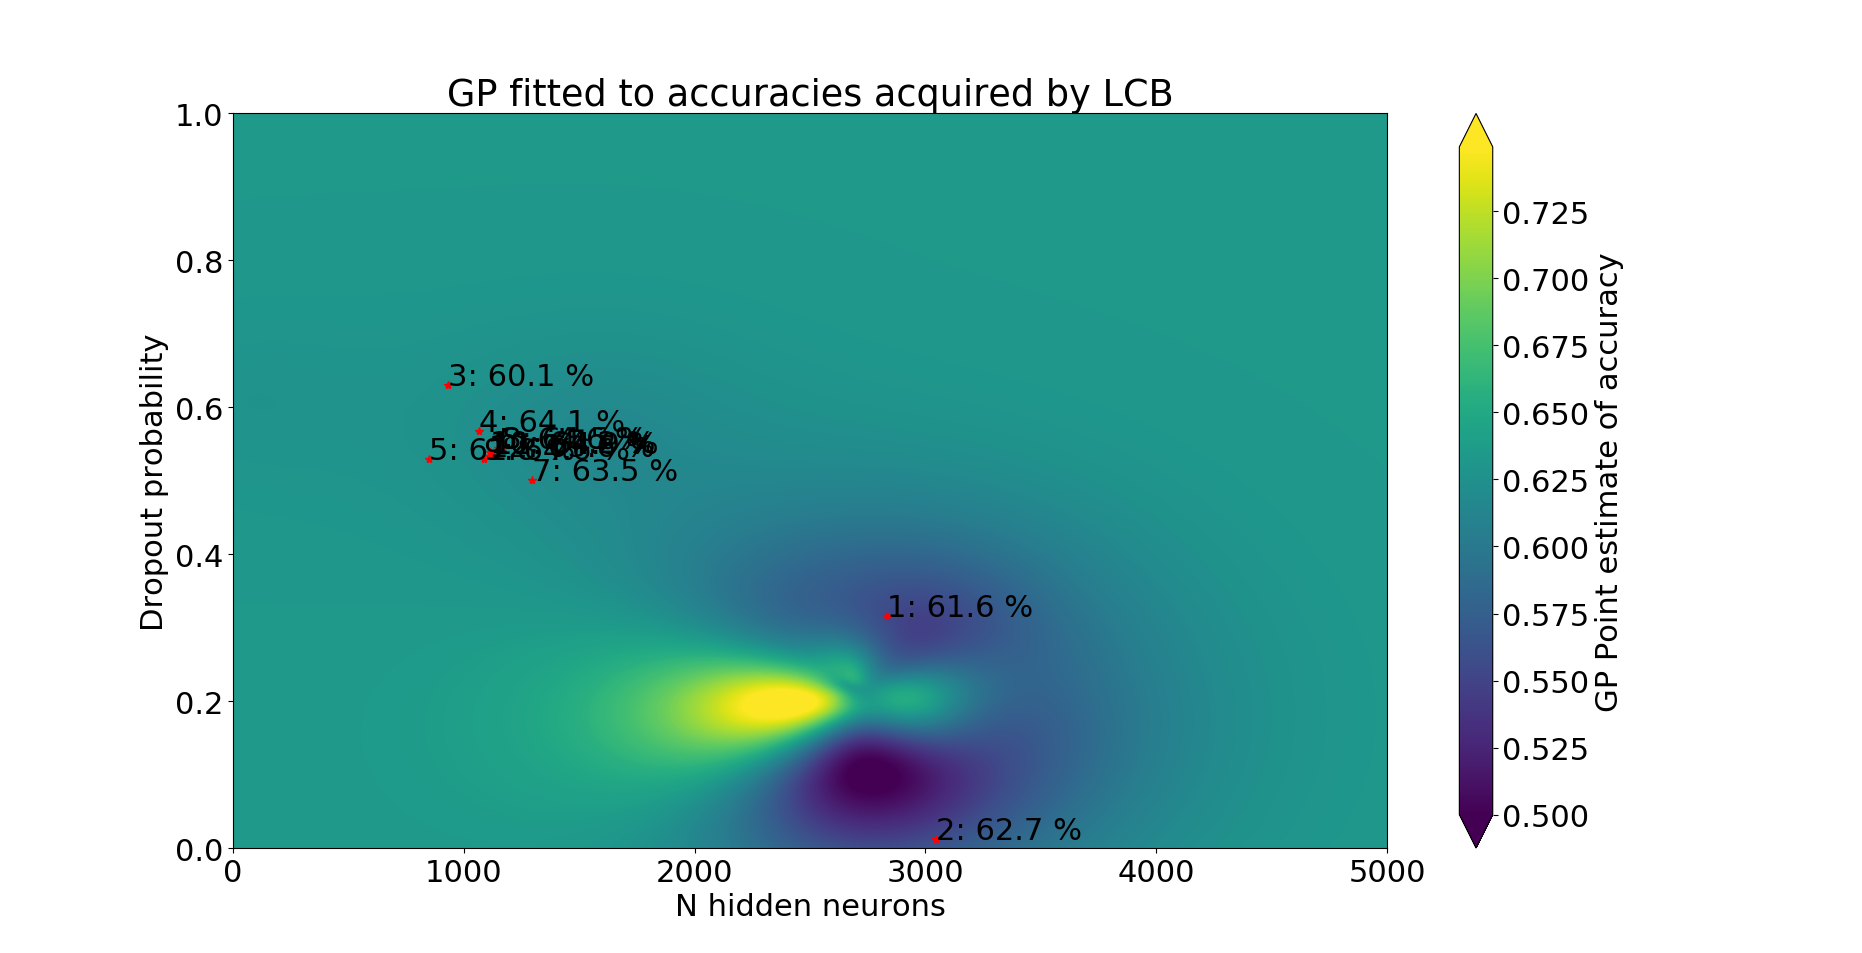
\includegraphics[width=\textwidth]{LCBGP}	

\end{figure}
\begin{table}[H]
	\caption{Bayesian optimization with EI as acquisition function \label{EI}}
	\centering
	\begin{tabular}{|l|l|l|l|l|}
		\hline
		Iteration & Hidden units & Dropout probability & Activation function & Accuracy \\ \hline
		1 & 3917 & 0.6923 & ReLU & 0.5165 \\ \hline 

		2 & 1805 & 0.1127 & Tanh & 0.6091 \\ \hline 

		3 & 1217 & 0.7398 & ReLU6 & 0.5765 \\ \hline 

		4 & 2618 & 0.6605 & ReLU & 0.5605 \\ \hline 

		5 & 2639 & 0.491 & Tanh & 0.6115 \\ \hline 

		6 & 2220 & 0.3325 & Tanh & 0.6185 \\ \hline 

		7 & 1002 & 0.4978 & Tanh & 0.5965 \\ \hline 

		8 & 3354 & 0.1637 & Tanh & 0.6091 \\ \hline 

		9 & 1 & 0.1262 & ReLU & 0.1145 \\ \hline 

		10 & 2863 & 0.5179 & Tanh & 0.5595 \\ \hline 

		11 & 2540 & 0.1569 & Tanh & 0.6275 \\ \hline 

		12 & 3251 & 1.0 & ReLU6 & 0.0835 \\ \hline 

	\end{tabular}
\end{table}
\begin{table}[H]
	\caption{Bayesian optimization with MPI as acquisition function \label{MPI}}
	\centering
	\begin{tabular}{|l|l|l|l|l|}
		\hline
		Iteration & Hidden units & Dropout probability & Activation function & Accuracy \\ \hline
1 & 2403 & 0.6196 & Sigmoid & 0.647 \\ \hline 

2 & 130 & 0.7724 & ReLU & 0.202 \\ \hline 

3 & 2706 & 0.4818 & Tanh & 0.5685 \\ \hline 

4 & 554 & 0.03571 & ReLU6 & 0.6245 \\ \hline 

5 & 2983 & 0.5369 & ReLU & 0.6145 \\ \hline 

6 & 2397 & 0.6166 & Sigmoid & 0.6275 \\ \hline 

7 & 2407 & 0.6219 & Sigmoid & 0.6385 \\ \hline 

8 & 2471 & 0.6537 & Sigmoid & 0.6435 \\ \hline 

9 & 2601 & 0.7138 & Sigmoid & 0.6367 \\ \hline 

10 & 3794 & 0.4693 & ReLU & 0.6113 \\ \hline 

11 & 2641 & 0.6416 & Sigmoid & 0.6285 \\ \hline 

12 & 2176 & 0.69 & Sigmoid & 0.6355 \\ \hline 

	\end{tabular}
\end{table}



\begin{table}[H]
	\caption{Bayesian optimization with LCB as acquisition function \label{LCB}}
	\centering
	\begin{tabular}{|l|l|l|l|l|}
		\hline
		Iteration & Hidden units & Dropout probability & Activation function & Accuracy \\ \hline
		1 & 2835 & 0.316 & ReLU6 & 0.6162 \\ \hline 
		2 & 3046 & 0.01182 & Sigmoid & 0.627 \\ \hline 
		3 & 934 & 0.6308 & Tanh & 0.6005 \\ \hline 
		4 & 1068 & 0.5681 & Sigmoid & 0.641 \\ \hline 
		5 & 848 & 0.5295 & ReLU & 0.6175 \\ \hline 
		6 & 1150 & 0.5441 & Sigmoid & 0.646 \\ \hline 
		7 & 1297 & 0.5009 & Sigmoid & 0.635 \\ \hline 
		8 & 1165 & 0.5443 & Sigmoid & 0.6455 \\ \hline 
		9 & 1089 & 0.5296 & Sigmoid & 0.646 \\ \hline 
		10 & 1115 & 0.5386 & Sigmoid & 0.6425 \\ \hline 
		11 & 1127 & 0.5375 & Sigmoid & 0.649 \\ \hline 
		12 & 1112 & 0.5333 & Sigmoid & 0.636 \\ \hline 
	\end{tabular}
\end{table}
 
 
\begin{table}[H]
	\caption{Grid search \label{grid}}
	\centering
	\begin{tabular}{|l|l|l|l|l|}
		\hline
		Iteration & Hidden units & Dropout probability & Activation function & Validation loss \\ \hline
		1         & 100          & 0.33                & Sigmoid             & 0.6345          \\ \hline
		2         & 100          & 0.33                & Sigmoid             & 0.6405          \\ \hline
		3         & 100          & 0.66                & ReLU                & 0.5150          \\ \hline
		4         & 100          & 0.66                & Sigmoid             & 0.5610          \\ \hline
		5         & 2000         & 0.33                & Tanh                & 0.513           \\ \hline
		6         & 2000         & 0.33                & ReLU                & 0.649           \\ \hline
		7         & 2000         & 0.66                & Sigmoid             & 0.6525          \\ \hline
		8         & 2000         & 0.66                & ReLU6               & 0.5685          \\ \hline
		9         & 4000         & 0.33                & Tanh                & 0.5595          \\ \hline
		10        & 4000         & 0.33                & ReLU6               & 0.5345          \\ \hline
		11        & 4000         & 0.66                & ReLU6               & 0.5015          \\ \hline
		12        & 4000         & 0.66                & Tanh                & 0.5050          \\ \hline
	\end{tabular}
\end{table}

\end{document}

















